\documentclass[12pt]{beamer}

\usepackage{epstopdf}
\usepackage{helvet}
\usepackage{graphicx}
\usepackage{caption}
\usepackage{subcaption}
\usepackage{tikz}

\usepackage{hyperref}
\usepackage{listings}



\usebackgroundtemplate



\usetikzlibrary{shapes,arrows}
\usetheme{Berlin}
\setbeamertemplate{navigation symbols}{}
\setbeamersize{text margin left = 6mm, text margin right = 6mm} 


%%%%%%%%%%%%%%%%%%%%%%%%%%%%%%%%%%%%%%%%%%%%%%%%%%%%%%%%%%%%%%%%%%%%%%%%%%%%%%%%
%%%%%%%%%%%%%%%%%%%%%%%%%%%%%%%%%%%%%%%%%%%%%%%%%%%%%%%%%%%%%%%%%%%%%%%%%%%%%%%%
%%
%%   COVER SLIDE
%%
%%%%%%%%%%%%%%%%%%%%%%%%%%%%%%%%%%%%%%%%%%%%%%%%%%%%%%%%%%%%%%%%%%%%%%%%%%%%%%%%
\title{\sc  Artificial Neural Networks}
\subtitle{\sc Brown Bag} 
%%%%%%%%%%%%%%%%%%%%%%%%%%%%%%%%%%%%%%%%%%%%%%%%%%%%%%%%%%%%%%%%%%%%%%%%%%%%%%%%
%%
%%   CONTENTS SLIDE
%%
%%%%%%%%%%%%%%%%%%%%%%%%%%%%%%%%%%%%%%%%%%%%%%%%%%%%%%%%%%%%%%%%%%%%%%%%%%%%%%%%
\begin{document}
\begin{frame}
\maketitle
\end{frame}
\begin{frame}{\sc Contents}
\begin{center}
\tableofcontents
\end{center}
\end{frame}

%%%%%%%%%%%%%%%%%%%%%%%%%%%%%%%%%%%%%%%%%%%%%%%%%%%%%%%%%%%%%%%%%%%%%%%%%%%%%%%%
%%
%%   INTRODUCTION 
%%
%%%%%%%%%%%%%%%%%%%%%%%%%%%%%%%%%%%%%%%%%%%%%%%%%%%%%%%%%%%%%%%%%%%%%%%%%%%%%%%%
\section{\sc Introduction}


\begin{frame}{\sc Introduction Slide}
\begin{center}

{\sl How do you write a program to read this?}


\begin{figure}[ht]
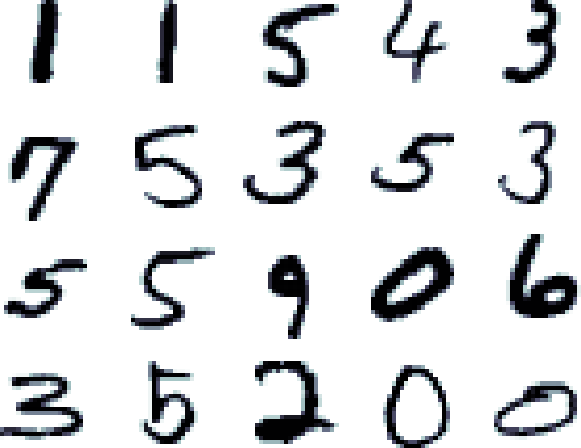
\includegraphics[scale=0.5]{figures/mnist_originals.png}
\end{figure}


\end{center}
\end{frame}

%%%%%%%%%%%%%%%%%%%%%%%%%%%%%%%%%%%%%%%%%%%%%%%%%%%%%%%%%%%%%%%%%%%%%%%%%%%%%%%%

\begin{frame}{\sc So how do we teach computers?}

\begin{columns}

\column{2.4in}
\begin{figure}
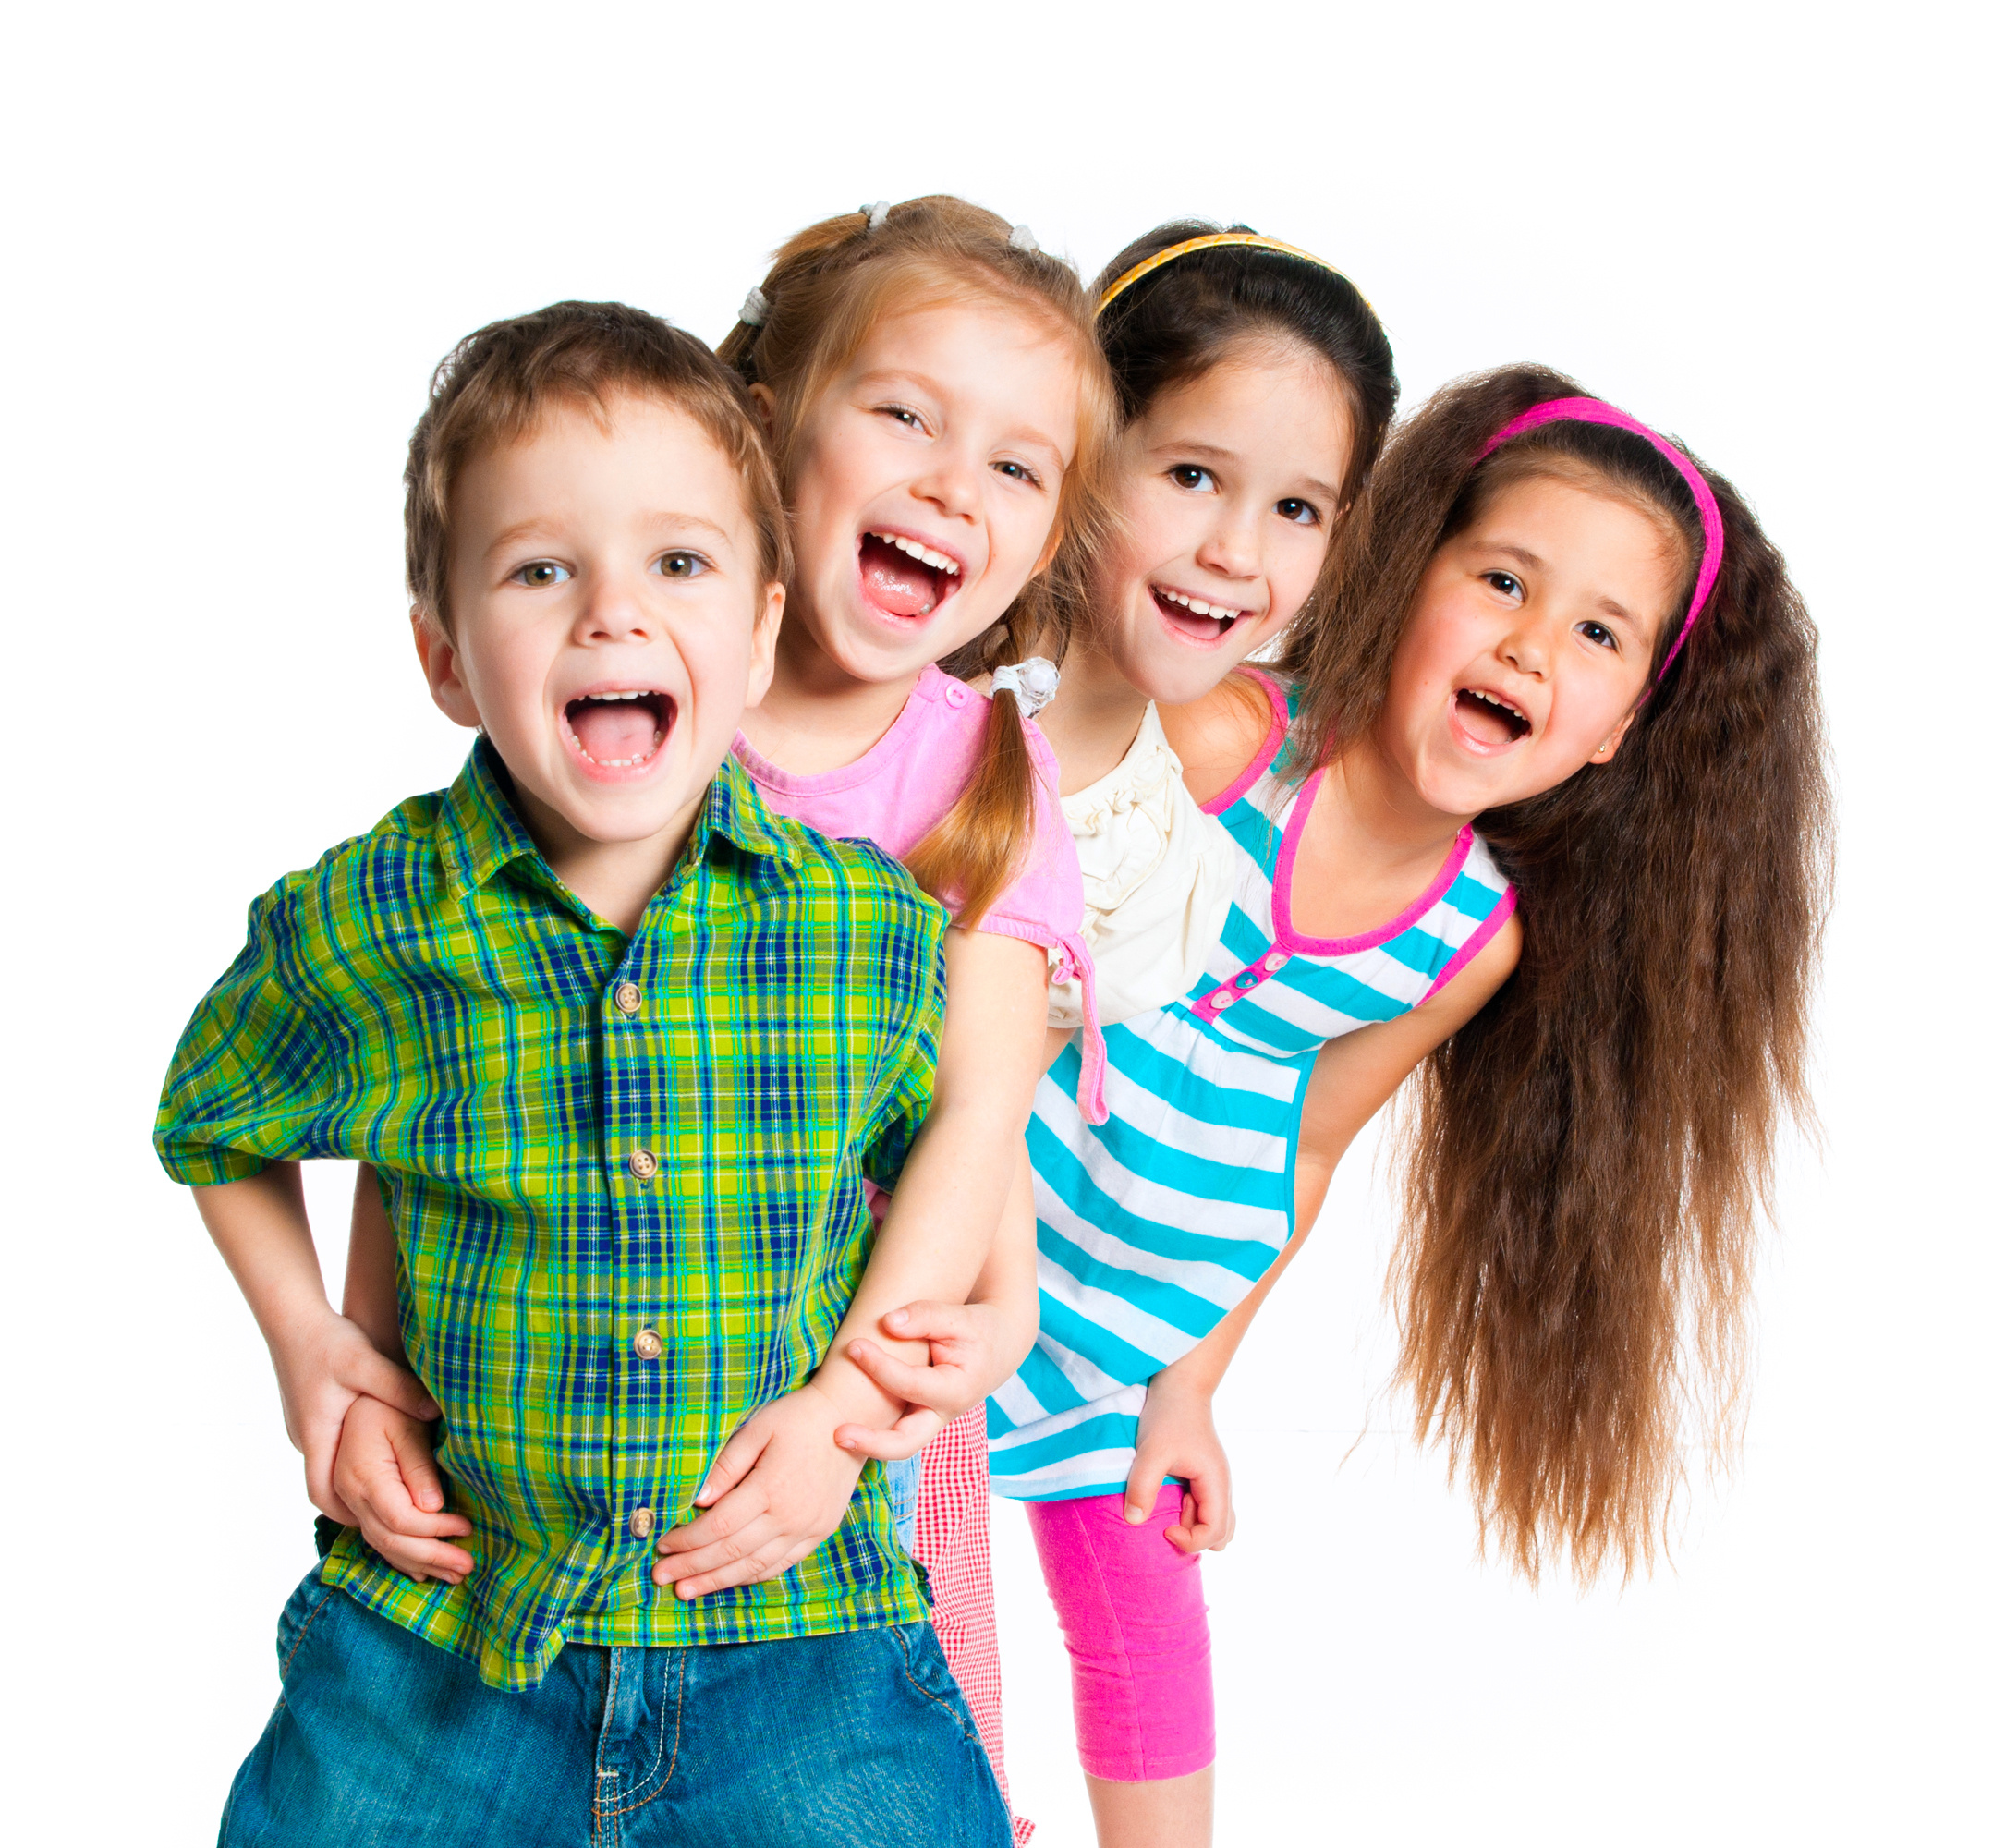
\includegraphics[scale=0.3]{figures/kids}
\end{figure}


\column{2in}
{\sc Consequences}
\begin{itemize}
\item Simpler signal represntation 
\item Reduced computational demands
\item Efficient processing 
\item Portable and affordable BCIs
\end{itemize}

\end{columns}

\end{frame}


%%%%%%%%%%%%%%%%%%%%%%%%%%%%%%%%%%%%%%%%%%%%%%%%%%%%%%%%%%%%%%%%%%%%%%%%%%%%%%%%
%%
%%   BACKGROUND 
%%
%%%%%%%%%%%%%%%%%%%%%%%%%%%%%%%%%%%%%%%%%%%%%%%%%%%%%%%%%%%%%%%%%%%%%%%%%%%%%%%%
\section{\sc Background}


\begin{frame}{\sc A brief intro to brain matters}
\begin{center}

\begin{figure}[ht]
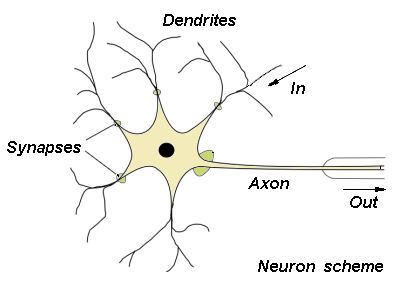
\includegraphics[scale=1]{figures/neuron.png}
\end{figure}

\end{center}
\end{frame}


%%%%%%%%%%%%%%%%%%%%%%%%%%%%%%%%%%%%%%%%%%%%%%%%%%%%%%%%%%%%%%%%%%%%%%%%%%%%%%%%


\begin{frame}{\sc Another Background Slide}
\begin{center}




\end{center}
\end{frame}




%%%%%%%%%%%%%%%%%%%%%%%%%%%%%%%%%%%%%%%%%%%%%%%%%%%%%%%%%%%%%%%%%%%%%%%%%%%%%%%%
%%
%%   METHODOLOGY
%%
%%%%%%%%%%%%%%%%%%%%%%%%%%%%%%%%%%%%%%%%%%%%%%%%%%%%%%%%%%%%%%%%%%%%%%%%%%%%%%%%

\section{\sc Methodology}

\begin{frame}{\sc This is the Methodology of my stuff}

\end{frame}

%%%%%%%%%%%%%%%%%%%%%%%%%%%%%%%%%%%%%%%%%%%%%%%%%%%%%%%%%%%%%%%%%%%%%%%%%%%%%%%%


\begin{frame}[fragile]
\frametitle{\sc P300 Speller}



\lstdefinestyle{customc}{
  belowcaptionskip=1\baselineskip,
  breaklines=true,
  frame=L,
  xleftmargin=\parindent,
  language=LaTeX,
  showstringspaces=false,
  basicstyle=\footnotesize\ttfamily,
  keywordstyle=\bfseries\color{green!40!black},
  commentstyle=\itshape\color{purple!40!black},
  identifierstyle=\color{blue},
  stringstyle=\color{orange},
}

\begin{center}
This is code to embed a video in your presentation. 

\begin{lstlisting}

\begin{figure}[ht]
\includemovie[
poster,
text={\small(Loading...)}
]{6cm}{6cm}{P300.mp4}
\end{figure}


\end{lstlisting}

\end{center}

\end{frame}






%%%%%%%%%%%%%%%%%%%%%%%%%%%%%%%%%%%%%%%%%%%%%%%%%%%%%%%%%%%%%%%%%%%%%%%%%%%%%%%%
%%
%%   RESULTS
%%
%%%%%%%%%%%%%%%%%%%%%%%%%%%%%%%%%%%%%%%%%%%%%%%%%%%%%%%%%%%%%%%%%%%%%%%%%%%%%%%%
\section{\sc Results}


\begin{frame}{\sc Results, Show Me the Money}



\end{frame}



%%%%%%%%%%%%%%%%%%%%%%%%%%%%%%%%%%%%%%%%%%%%%%%%%%%%%%%%%%%%%%%%%%%%%%%%%%%%%%%%
%%
%%   CONCLUSION
%%
%%%%%%%%%%%%%%%%%%%%%%%%%%%%%%%%%%%%%%%%%%%%%%%%%%%%%%%%%%%%%%%%%%%%%%%%%%%%%%%%


\section{\sc Conclusion}


\begin{frame}{\sc To Conclude}

\begin{columns}

\column{2.4in}
{\sc Results}
\begin{itemize}
\item The usefull information is not lost with signal distortion 
\item Counter-intuitive result
\item Indication of a some hidden process
\item EEG signals can be represented in simpler forms 
\end{itemize}

\column{2in}
{\sc Consequences}
\begin{itemize}
\item Simpler signal represntation 
\item Reduced computational demands
\item Efficient processing 
\item Portable and affordable BCIs
\end{itemize}

\end{columns}

\end{frame}

%%%%%%%%%%%%%%%%%%%%%%%%%%%%%%%%%%%%%%%%%%%%%%%%%%%%%%%%%%%%%%%%%%%%%%%%%%%%%%%%


\begin{frame}[fragile]
\frametitle{\sc Columns Code}


\begin{lstlisting}
\begin{columns}
\column{2.4in}{\sc Results}
\begin{itemize}
\item One
\item Two
\end{itemize}
\column{2in}{\sc Consequences}
\begin{itemize}
\item Other one
\end{itemize}
\end{columns}


\end{lstlisting}


\end{frame}

%%%%%%%%%%%%%%%%%%%%%%%%%%%%%%%%%%%%%%%%%%%%%%%%%%%%%%%%%%%%%%%%%%%%%%%%%%%%%%%%
%%
%%  DISCUSSION
%%
%%%%%%%%%%%%%%%%%%%%%%%%%%%%%%%%%%%%%%%%%%%%%%%%%%%%%%%%%%%%%%%%%%%%%%%%%%%%%%%%
\section{\sc Discussion}


\begin{frame}{\sc Let`s Talk}


\begin{center}
These results can provide further insight into brain functionality
\end{center}




\end{frame}

%%%%%%%%%%%%%%%%%%%%%%%%%%%%%%%%%%%%%%%%%%%%%%%%%%%%%%%%%%%%%%%%%%%%%%%%%%%%%%%%
%%
%%  ACKNOWLEDGEMENTS
%%
%%%%%%%%%%%%%%%%%%%%%%%%%%%%%%%%%%%%%%%%%%%%%%%%%%%%%%%%%%%%%%%%%%%%%%%%%%%%%%%%
\section{\sc Section}

\begin{frame}{\sc I would like to thank...}

\end{frame}


%%%%%%%%%%%%%%%%%%%%%%%%%%%%%%%%%%%%%%%%%%%%%%%%%%%%%%%%%%%%%%%%%%%%%%%%%%%%%%%%


\begin{frame}{\sc Questions?}

\begin{center}
Here you can have pictures of the investigator and mentor, os the logos of the labs and institutions involved
\end{center}

\end{frame}




\end{document}